\documentclass[tikz,border=5pt]{standalone}
\pdfinfoomitdate=1
\pdftrailerid{}
\pdfsuppressptexinfo=-1
\usepackage{pgfplots}
\usepgfplotslibrary{groupplots}
\pgfplotsset{compat=1.18}
\definecolor{atlasBlue}{HTML}{0072B2}
\definecolor{atlasOrange}{HTML}{E69F00}
\definecolor{atlasGreen}{HTML}{009E73}
\definecolor{atlasPurple}{HTML}{CC79A7}
\definecolor{atlasGray}{HTML}{777777}
% NATO SERS figure F47; data_sha256=efc210af3c98327045e51be6c5055aecf6bd8aea17e6d987ac3b96d93cd7fe6f
% title=Recorded field-trial detection completeness and model agreement
% caption=Recorded field-log outcomes at the master-substrate-instrument-view unit for C-SELECTED PP-U-MIN held predictions. Points are complete-case recorded detection/specificity; horizontal bars are worst-to-best bounds for genuinely missing logs, not confidence intervals. M and conflicting repeats are excluded from the definite endpoint. Agreement compares recorded success/failure with correct/incorrect analyte classification.
\begin{document}
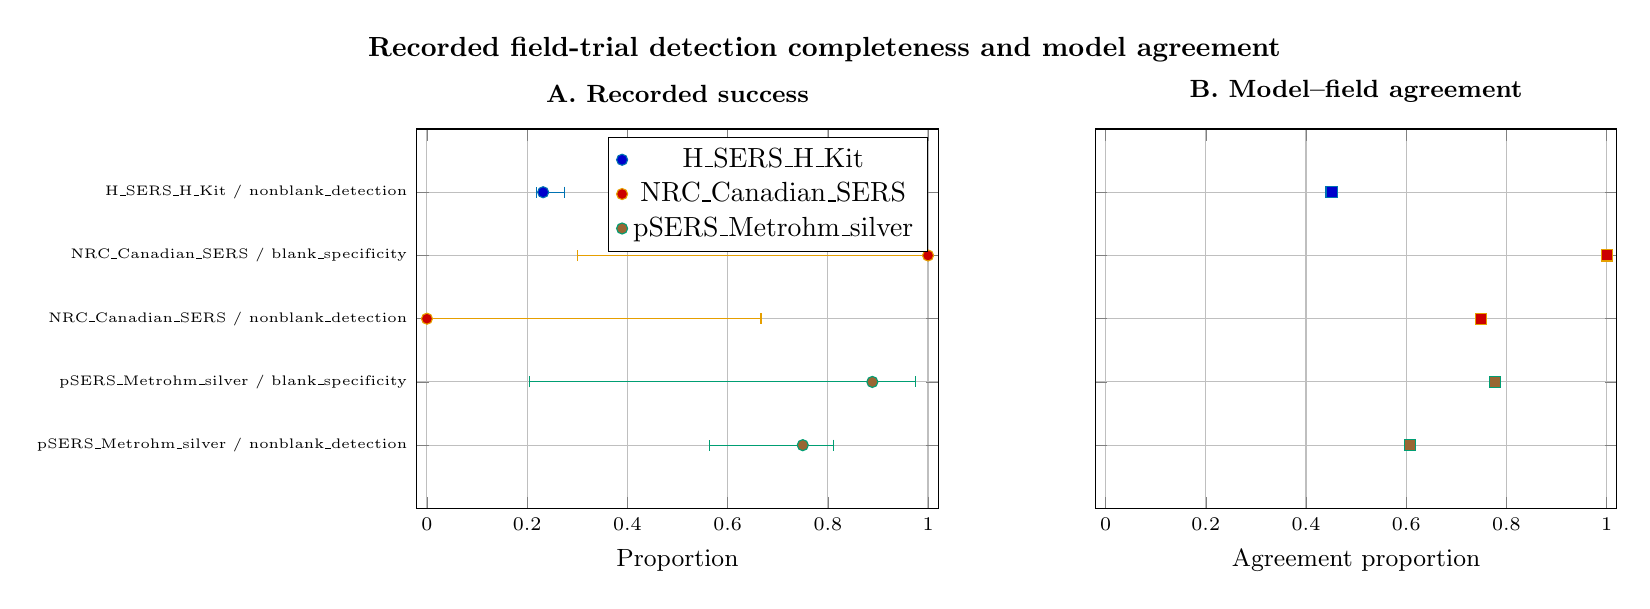
\begin{tikzpicture}
\begin{groupplot}[group style={group size=2 by 1,horizontal sep=2.0cm},width=8.2cm,height=6.4cm,
tick label style={font=\scriptsize},label style={font=\small},title style={font=\small\bfseries},
ytick={4,3,2,1,0},yticklabels={H\_SERS\_H\_Kit / nonblank\_detection,NRC\_Canadian\_SERS / blank\_specificity,NRC\_Canadian\_SERS / nonblank\_detection,pSERS\_Metrohm\_silver / blank\_specificity,pSERS\_Metrohm\_silver / nonblank\_detection},y tick label style={font=\tiny,align=right},grid=major]
\nextgroupplot[title={A. Recorded success},xlabel={Proportion},xmin=-0.02,xmax=1.02,ymin=-1,ymax=5]
\addplot+[only marks,mark=*,color=atlasBlue,error bars/.cd,x dir=both,x explicit] coordinates {(0.23188406,4) += (0.042088545,0) -= (0.012705976,0)};\addlegendentry{H\_SERS\_H\_Kit}
\addplot+[only marks,mark=*,color=atlasOrange,error bars/.cd,x dir=both,x explicit] coordinates {(1,3) += (0,0) -= (0.7,0) (0,2) += (0.66666667,0) -= (0,0)};\addlegendentry{NRC\_Canadian\_SERS}
\addplot+[only marks,mark=*,color=atlasGreen,error bars/.cd,x dir=both,x explicit] coordinates {(0.88888889,1) += (0.085470085,0) -= (0.68376068,0) (0.75,0) += (0.062030075,0) -= (0.18609023,0)};\addlegendentry{pSERS\_Metrohm\_silver}
\nextgroupplot[title={B. Model--field agreement},xlabel={Agreement proportion},xmin=-0.02,xmax=1.02,ymin=-1,ymax=5,yticklabels={}]
\addplot+[only marks,mark=square*,color=atlasBlue] coordinates {(0.45098039,4)};
\addplot+[only marks,mark=square*,color=atlasOrange] coordinates {(1,3) (0.75,2)};
\addplot+[only marks,mark=square*,color=atlasGreen] coordinates {(0.77777778,1) (0.60810811,0)};
\end{groupplot}
\node[font=\normalsize\bfseries,anchor=south] at (current bounding box.north) {Recorded field-trial detection completeness and model agreement};
\end{tikzpicture}
\end{document}
